
\overlays{8}{%
  \begin{slide}{Das Fahrerinterface}
      \begin{minipage}{7.0cm}
        \untilSlide*{4}{%
          Gr�nde f�r einen PDA:
          \begin{itemize}
            \fromSlide{2}{\item Gen�gend Rechenleistung (Hochsprachen)}%
            \fromSlide{3}{\item Display (Warnhinweise)}%
            \fromSlide{4}{\item Interaktion (Einstellungen, Routing, etc.)}%
          \end{itemize}
        }
      \fromSlide*{5}{%
        Gr�nde f�r \emph{diesen} PDA
        \begin{itemize}
          \fromSlide{6}{\item Display}%
          \fromSlide{7}{\item Rechenleistung}%
          \fromSlide{8}{\item Linux (Multitasking, Programmierung)}%
        \end{itemize}
      }
    \end{minipage}
%
    \begin{minipage}{3cm}
      \begin{center}
        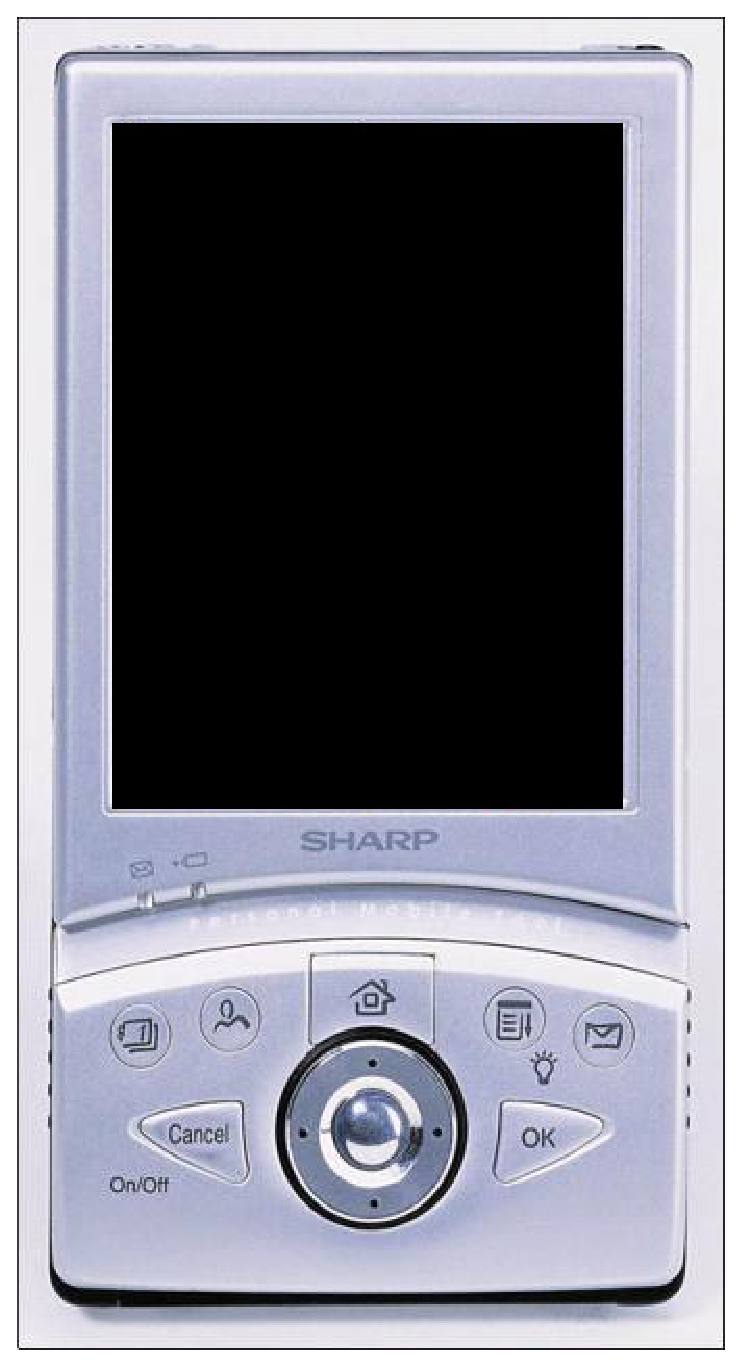
\includegraphics[width=3cm]{zaurus.eps}
      \end{center}
    \end{minipage}
  \end{slide}
}


% ============================================================


\overlays{5}{
  \begin{slide}{DPI aus Entwicklersicht}
    \untilSlide*{1}{
      \begin{center}
        
\includegraphics[width=8cm]{zustaende.eps}\\
        Informal: Konzept der kommunizierenden Automaten
      \end{center}
    }
    \fromSlide{2}{
      Vaterklasse \texttt{Driver} f�r alle Treiber
      \begin{itemize}
        \fromSlide{3}{\item GUI ruft \texttt{Blinken()} des Treibers
          auf.}
        \fromSlide{4}{\item \texttt{send(Message)}: Versenden von
          \emph{Nachrichten}.}
        \fromSlide{5}{\item \texttt{receive(Message)}: Empfang von
          Nachrichten.}
      \end{itemize}
    }
  \end{slide}
}


% ============================================================


\overlays{3}{%
  \begin{slide}{Weg der Nachricht durch das DPI}
    \begin{itemstep}
    \item \texttt{Driver.send()} �berpr�ft die Nachricht
    \item \texttt{message\_dispatcher.send()} sendet auf passendem
      \texttt{bus\_manager} heraus $\to$ Indirektion
    \item \texttt{bus\_manager.send()} sendet auf passendem
      \texttt{bus} heraus $\to$ Indirektion
    \end{itemstep}
  \end{slide}
}